% !TeX program = xelatex
\documentclass[12pt,a4paper]{article}

%  Базовые пакеты 
\usepackage{geometry}
\geometry{margin=2.5cm}
\usepackage{fontspec}
\setmainfont{Times New Roman}
\usepackage{polyglossia}
\setdefaultlanguage{russian}
\usepackage{setspace}
\onehalfspacing
\usepackage{hyperref}
\hypersetup{
  unicode=true,
  colorlinks=true,
  linkcolor=black,
  urlcolor=blue,
  citecolor=black,
  pdftitle={Эволюция методов: от ARIMA и экспоненциального сглаживания до LSTM и трансформеров}
}

\usepackage{amsmath,amssymb,mathtools}
\usepackage{bm}
% операторы
\DeclareMathOperator{\Var}{Var}
\DeclareMathOperator{\Cov}{cov}

\setcounter{tocdepth}{2}

\title{\textbf{Эволюция методов: от ARIMA и экспоненциального сглаживания до LSTM и трансформеров}}
\date{\the\year}

\begin{document}

%  Титульный лист 
\pagenumbering{gobble}
\begin{titlepage}
    \centering
    \vspace*{1cm}
    {\large Санкт-Петербургский государственный университет\par}
    {\large Математико-механический факультет\par}
    {\large Искусственный интеллект и наука о данных\par}
    \vfill
    {\Large Доклад на тему}\par
    \vspace{0.8cm}
    {\LARGE \textbf{Эволюция методов: от ARIMA и экспоненциального сглаживания до LSTM и трансформеров}}\par
    \vfill
    \begin{flushleft}
        \textbf{Автор:} Мурадян Денис Степанович\\[2pt]
        \textbf{Уровень:} Бакалавриат, 3 курс\\[2pt]
        \textbf{Дисциплина:} Машинное обучение\\[2pt]
    \end{flushleft}
    \vspace{0.8cm}
    {\large \the\year\par}
\end{titlepage}

%  Аннотация 
\pagenumbering{arabic}
\section{Аннотация}

Доклад посвящён развитию подходов к прогнозированию временных рядов. Рассматривается переход от традиционных статистических моделей к современным архитектурам машинного обучения, способным учитывать нелинейные зависимости и сложную динамику данных. Последовательно анализируются основные этапы эволюции методов, приводятся ключевые идеи и математические основы, на которых они построены. Особое внимание уделяется тому, как развитие моделей отражает расширение возможностей анализа временных данных и повышение точности прогнозов.

\medskip
\subsection{\textbf{Задачи:}}
\begin{enumerate}
    \item Сформулировать задачу прогнозирования временных рядов и описать её основные элементы.
    \item Рассмотреть классические статистические подходы: скользящее среднее, экспоненциальное сглаживание, модели Холта и Хольта–Уинтерса, а также семейство авторегрессионных моделей AR, MA, ARMA, ARIMA и их сезонные расширения.
    \item Показать, какие ограничения традиционных методов послужили стимулом к появлению машинного обучения и нейросетевых моделей.
    \item Разобрать рекуррентные нейронные сети (RNN), их модификации LSTM и GRU, объяснив принципы работы и особенности применения к временным данным.
    \item Рассмотреть механизм внимания и архитектуры типа \textit{sequence-to-sequence}, показать, как они решают проблему ограниченного контекста в рекуррентных моделях.
    \item Рассмотреть архитектуру \textit{transformers} как современное развитие идей анализа последовательностей и описать роль self-attention в обработке временных зависимостей.
    \item Обозначить основные метрики качества прогнозов и принципы оценки моделей.
    \item Привести краткий обзор научных источников и примеры актуальных наборов данных, применяемых в данной области.
\end{enumerate}

%  Содержание 
\clearpage
\tableofcontents
\thispagestyle{plain}


%  Раздел 1. Введение 
\clearpage
\pagenumbering{arabic}

\section{Введение} 

\subsection{Определение временного ряда}
Временной ряд - это последовательность наблюдений некоторого признака, упорядоченных во времени. Каждое значение такого признака зависит от момента наблюдения и обозначается через~$y_t$, где~$t$ - номер или метка времени.
Примерами временных рядов могут быть динамика температуры воздуха, объёмы продаж товаров по дням, уровень потребления электроэнергии или колебания курсов валют.

Временные ряды позволяют анализировать закономерности во времени: наличие тренда, сезонных колебаний, а также случайных компонент, возникающих под воздействием внешних факторов. Цель прогнозирования состоит в том, чтобы на основе имеющихся данных предсказать будущие значения ряда.

\subsection{Постановка задачи прогнозирования}
Пусть задан временной ряд
\[
(y_t,\; t\in\mathbb{N}),
\]
для которого известны значения $y_1,\,y_2,\,\ldots,\,y_T$.
Требуется построить функцию прогнозирования~$f$, обеспечивающую приближение будущих значений:
\[
\hat{y}_{T+h}=f(y_1,\,y_2,\,\ldots,\,y_T,\,h),
\]
где $h\in\{1,\ldots,H\}$ - шаг прогноза, а $H$ - горизонт прогнозирования.
Иными словами, прогноз значения ряда в момент времени $T+h$ строится на основе известных наблюдений до момента~$T$.

Помимо точечного прогноза, часто рассматривается предсказательный интервал
\[
(d_{T+h},\,u_{T+h}),
\]
для которого выполняется условие
\[
P\!\left(d_{T+h}\le y_{T+h}\le u_{T+h}\right)\ge \alpha,
\]
где~$\alpha$ - доверительная вероятность. Такой интервал отражает неопределённость прогноза.

\subsection{Иллюстративный пример}
Рассмотрим ситуацию, когда $y_t$ обозначает значение некоторого показателя в день~$t$, и известны наблюдения за месяц:
\[
y_1,\,y_2,\,\ldots,\,y_{30}.
\]
Требуется спрогнозировать значения на неделю вперёд.
Тогда прогноз на один день вперёд:
\[
\hat{y}_{31}=f(y_1,\,\ldots,\,y_{30},\,1),
\]
а прогноз на пятый день вперёд:
\[
\hat{y}_{35}=f(y_1,\,\ldots,\,y_{30},\,5).
\]
Если впоследствии появляются новые данные, прогноз можно обновить, например:
\[
\hat{y}_{35}=f(y_1,\,\ldots,\,y_{33},\,2),
\]
что соответствует уточнённому прогнозу, построенному в момент времени~$33$.

Иногда указывают, в какой момент был сформирован прогноз:
\[
\hat{y}_{35|30} \quad\text{или}\quad \hat{y}_{35|33},
\]
что означает прогноз на $35$-й день, построенный соответственно на $30$-й или $33$-й день.

\subsection{Многомерные и вспомогательные признаки}
Если одновременно наблюдаются несколько показателей, прогноз может строиться только для части из них - так называемых целевых признаков. Остальные характеристики могут использоваться как вспомогательные, повышающие точность прогноза.
Например, при моделировании спроса на товар в магазине полезно учитывать не только прошлые продажи, но и такие признаки, как день недели, месяц, сезон или наличие праздников.

\subsection{Практические примеры}
\begin{itemize}
    \item Прогноз температуры воздуха или осадков на несколько дней вперёд.
    \item Прогноз объёма продаж товара по неделям.
    \item Прогноз потребления электроэнергии по часам для планирования нагрузки энергосистемы.
\end{itemize}

\subsection{Формулировка в виде задачи регрессии}
Во многих случаях прогнозирование можно рассматривать как задачу регрессии.
Если функция $f$ использует только последние $p$ наблюдений, модель можно записать как
\[
y_t = f(y_{t-1},\,y_{t-2},\,\ldots,\,y_{t-p}),
\]
где $p$ - длина окна, задающая количество прошлых значений, необходимых для прогноза.
Функцию $f$ можно аппроксимировать различными методами: линейной или полиномиальной регрессией, деревьями решений, бустингом, рекуррентными или сверточными нейронными сетями и другими подходами машинного обучения.

При построении модели важно учитывать, какие данные доступны на момент времени~$t$. На практике это определяет, какие признаки могут быть использованы при обучении модели и при формировании прогноза.

\bigskip
Таким образом, задача прогнозирования временных рядов заключается в поиске зависимости между прошлыми и будущими значениями ряда. В следующих разделах будут рассмотрены основные методы, с помощью которых эта зависимость моделируется.





\section{Классические статистические подходы к прогнозированию временных рядов}

Классические статистические методы строятся вокруг простой, но мощной идеи: текущее значение временного ряда обычно связано со своим прошлым. Мы стремимся извлечь закономерности в уровне, тренде и сезонности, а также понять, насколько наблюдения зависят друг от друга на различных лагах. В этом разделе последовательно рассмотрим сглаживания (скользящее среднее, экспоненциальное сглаживание, модели Холта и Хольта–Уинтерса) и авторегрессионные семейства (AR, MA, ARMA, ARIMA) вместе с сезонными и экзогенными расширениями. Такой маршрут позволяет переходить от быстрого и интуитивного описания «текущего состояния» к формальным моделям, способным давать как точечные, так и интервальные прогнозы.

\subsection{Наблюдаемое прошлое и скользящие признаки}

Для прогнозирования величины $y_t$ естественно использовать её прошлые значения $y_{t-1},\dots,y_{t-p}$. Вместо того чтобы включать десятки или сотни отдельных лагов, часто агрегируют недавнюю историю через \emph{скользящее окно}. Пусть $k$ - длина окна. Тогда простое скользящее среднее оценивает текущий уровень как
\[
\tilde y_t=\frac{1}{k}\sum_{i=0}^{k-1} y_{t-i}.
\]
При небольшом $k$ оценка быстро реагирует, но менее устойчива к шуму; при большом $k$ - сильнее сглаживает, но запаздывает на трендах. На окне можно вычислять и другие статистики: взвешенное среднее, медиану, минимум/максимум, стандартное отклонение, а также применять экспоненциальное сглаживание.

\subsection{Экспоненциальные сглаживания: уровень, тренд и сезонность}

Экспоненциальные сглаживания дают компактное динамическое описание \emph{уровня} ряда и, при необходимости, \emph{тренда} и \emph{сезонности}. Их удобно использовать как самостоятельные модели и как базовые линии для сравнения.

\subsubsection{Простое экспоненциальное сглаживание (SES)}
SES агрегирует всю предысторию с убывающими весами и особенно полезно, когда ряд не демонстрирует устойчивого тренда:
\[
\hat y_{t+1\,|\,t}=\alpha y_t+(1-\alpha)\,\hat y_{t\,|\,t-1}, \qquad \alpha\in(0,1).
\]
Здесь $\hat y_{t+1\,|\,t}$ - прогноз на шаг вперёд, $\alpha$ - параметр памяти: при больших значениях модель быстрее реагирует на изменения, при малых - сильнее сглаживает колебания.

\subsubsection{Модель Холта: добавляем линейный тренд}
Если уровень систематически растёт или падает, к сглаженному уровню добавляют сглаженный \emph{наклон}. В аддитивной форме:
\[
\ell_t=\alpha y_t+(1-\alpha)(\ell_{t-1}+b_{t-1}), \qquad
b_t=\beta(\ell_t-\ell_{t-1})+(1-\beta)b_{t-1},
\]
\[
\hat y_{t+h\,|\,t}=\ell_t+h\,b_t.
\]
Величины $\ell_t$ и $b_t$ интерпретируются соответственно как «текущий уровень» и «скорость изменения уровня».

\subsubsection{Модель Хольта–Уинтерса: учитываем сезонность}
При повторяющихся паттернах с периодом $m$ добавляют сезонную компоненту. В аддитивном варианте (амплитуда сезонности почти постоянна):
\[
\ell_t=\alpha (y_t-s_{t-m})+(1-\alpha)(\ell_{t-1}+b_{t-1}), \quad
b_t=\beta(\ell_t-\ell_{t-1})+(1-\beta)b_{t-1},
\]
\[
s_t=\gamma (y_t-\ell_t)+(1-\gamma)s_{t-m}, \qquad
\hat y_{t+h\,|\,t}=\ell_t+h\,b_t+s_{t+m_h}, \quad m_h=((h-1)\bmod m)+1.
\]
В мультипликативном варианте (амплитуда пропорциональна уровню):
\[
\ell_t=\alpha \frac{y_t}{s_{t-m}}+(1-\alpha)(\ell_{t-1}+b_{t-1}), \quad
b_t=\beta(\ell_t-\ell_{t-1})+(1-\beta)b_{t-1},
\]
\[
s_t=\gamma \frac{y_t}{\ell_t}+(1-\gamma)s_{t-m}, \qquad
\hat y_{t+h\,|\,t}=(\ell_t+h\,b_t)\,s_{t+m_h}.
\]
Практически: аддитивную форму выбирают при «похожей» абсолютной амплитуде по сезонам; мультипликативную - когда колебания растут вместе с уровнем.

\subsection{Диагностика зависимостей и подготовка к моделированию}

\subsubsection{Лаги и лаговый оператор}
Лаг $\tau$ - сдвиг на $\tau$ шагов назад. Удобно пользоваться оператором $L$: $Ly_t=y_{t-1}$, $L^k y_t=y_{t-k}$. Такая запись компактно выражает разности и сезонные сдвиги.

\subsubsection{Автокорреляция (ACF) и частичная автокорреляция (PACF)}
Автокорреляционная функция оценивает линейную зависимость между $y_t$ и $y_{t+\tau}$:
\[
r_\tau=\frac{\sum_{t=1}^{T-\tau}(y_t-\overline y)(y_{t+\tau}-\overline y)}{\sum_{t=1}^T (y_t-\overline y)^2}, \qquad
\overline y=\frac{1}{T}\sum_{t=1}^T y_t.
\]
Пики на лагах $m,2m,\dots$ указывают на сезонность с периодом $m$. PACF измеряет «чистый» вклад лага $\tau$, устраняя линейное влияние промежуточных лагов: для AR($p$) PACF резко затухает после $p$, для MA($q$) аналогично затухает ACF после $q$. Эти шаблоны служат первыми ориентирами при выборе порядков моделей.

\subsubsection{Стационарность}

Интуитивно стационарность означает, что «статистические свойства ряда не меняются при сдвиге по времени». Формально различают два уровня.

\paragraph{Стационарность в узком (строгом) смысле.}
Ряд $\{y_t\}$ называется стационарным в узком смысле, если для любых целых $t_1,\dots,t_n$ и любого целого $\tau$ векторы
\[
(y_{t_1+\tau},\dots,y_{t_n+\tau}) \quad\text{и}\quad (y_{t_1},\dots,y_{t_n})
\]
совпадают по распределению. То есть совместное распределение не меняется при любом сдвиге всех моментов времени на одно и то же число.

\paragraph{Стационарность в широком смысле.}
Ряд $\{y_t\}$ называется стационарным в широком смысле (ковариационно стационарным), если выполняются три условия:
\[
\mathbb{E}[y_t^2]<\infty \;\;\text{для любого } t, \qquad
\mathbb{E}[y_t]=\mu \;\;\text{(не зависит от } t),
\]
\[
\mathrm{cov}(y_{t+\tau},y_{s+\tau})=\mathrm{cov}(y_t,y_s)\;\;\text{для любых } t,s,\tau,
\]
то есть ковариация зависит только от лага, а не от абсолютного времени. В частности, автоковариация $\gamma(\tau)=\mathrm{cov}(y_t,y_{t+\tau})$ зависит лишь от $\tau$.

\paragraph{Связь определений при нормальности.}
Если любой конечномерный вектор $(y_{t_1},\dots,y_{t_n})$ имеет многомерное нормальное распределение, то стационарности в узком и в широком смыслах эквивалентны. Это связано с тем, что нормальное распределение полностью определяется своим математическим ожиданием и ковариационной матрицей.

\paragraph{Иллюстративный пример.}
Рассмотрим процесс
\[
y_t=\xi_1\cos t+\xi_2\sin t,
\]
где независимые случайные величины $\xi_1,\xi_2$ принимают значения $\pm 1$ с вероятностями $1/2$. Тогда
\[
\mathbb{E}[y_t]=0,\qquad
\mathrm{cov}(y_t,y_s)=\mathbb{E}[y_t y_s]=\cos t\cos s\,\mathrm{Var}(\xi_1)+\sin t\sin s\,\mathrm{Var}(\xi_2)=\cos(t-s),
\]
то есть ряд стационарен в широком смысле (среднее неизменно, автоковариация зависит только от разности $t-s$). Однако он \emph{не} стационарен в узком смысле: действительно, $y_0=\xi_1\in\{-1,1\}$, тогда как
\[
y_{\pi/4}=\tfrac{\sqrt{2}}{2}(\xi_1+\xi_2)\in\{-\sqrt{2},\,0,\,\sqrt{2}\},
\]
и распределения $y_0$ и $y_{\pi/4}$ различны.

\paragraph{Типовые примеры нестационарности.}
\begin{itemize}
  \item \textbf{Случайное блуждание:} $y_t=y_{t-1}+\varepsilon_t$, где $\{\varepsilon_t\}$ - белый шум. Хотя $\mathbb{E}[y_t]$ постоянно, дисперсия $\mathrm{Var}(y_t)$ неограниченно растёт, поэтому стационарности нет.
  \item \textbf{Линейный тренд:} $y_t=\alpha+\beta t+\varepsilon_t$. Математическое ожидание зависит от $t$ (меняется уровень), следовательно, ряд нестационарен.
  \item \textbf{Чистая сезонность:} $y_t=\sin t+\varepsilon_t$. Среднее $\mathbb{E}[y_t]=\sin t$ периодически меняется с $t$, поэтому стационарность нарушена.
\end{itemize}

\paragraph{Практическая роль предположения.}
Большинство авторегрессионных моделей (AR, ARMA) предполагают хотя бы ковариационную стационарность исходного процесса или его преобразований. Если стационарность нарушена, оценки параметров и стандартные формулы для дисперсии прогноза могут быть несостоятельны. На практике для приведения ряда к стационарности используют стабилизацию дисперсии (например, преобразование Бокса–Кокса) и дифференцирование: обычное $(1-L)y_t$ для тренда и сезонное $(1-L^m)y_t$ для периодических паттернов.

\subsubsection{Стабилизация масштаба и снятие нестационарности}
Для стабилизации дисперсии часто применяют преобразование Бокса–Кокса:
\[
z_t=
\begin{cases}
\displaystyle \frac{y_t^{\lambda}-1}{\lambda}, & \lambda\neq 0,\\[4pt]
\ln y_t, & \lambda=0.
\end{cases}
\]
Тренды и сезонность устраняют разностями:
\[
(1-L)y_t=y_t-y_{t-1}, \qquad (1-L^m)y_t=y_t-y_{t-m}.
\]
Обычно сначала делают сезонную разность $(1-L^m)$, затем при необходимости применяют обычную разность $(1-L)$ до тех пор, пока диаграммы ACF/PACF и тесты на стационарность не укажут на приемлемость предположений.

\subsection{Авторегрессионные семейства моделей}

После того как простые сглаживания позволяют понять тренды и сезонность, возникает вопрос: можно ли формально описать зависимость текущего значения ряда от его прошлых значений и случайных возмущений? Ответ дают \textbf{авторегрессионные} и \textbf{скользящие средние} модели, объединённые под общим названием ARIMA-семейства (от \textit{Autoregressive Integrated Moving Average}).

В отличие от методов сглаживания, которые эмпирически взвешивают прошлое, эти модели предполагают, что наблюдаемые данные - результат динамической стохастической системы, где каждое новое значение формируется как комбинация прошлых значений и случайных шумов.

\subsubsection{Основная идея и лаговая запись}

Для описания динамической зависимости вводится \emph{лаговый оператор} $L$, который сдвигает ряд во времени: $Ly_t = y_{t-1}$, $L^k y_t = y_{t-k}$.
Это позволяет записывать модели в компактной форме и понимать, какие лаги участвуют в прогнозе.

Две ключевые составляющие таких моделей:
\begin{itemize}
    \item \textbf{Авторегрессия (AR):} текущее значение зависит от нескольких предыдущих наблюдений ряда.
    \item \textbf{Скользящее среднее (MA):} текущее значение включает линейную комбинацию случайных шумов прошлых шагов.
\end{itemize}

\subsubsection{AR($p$): авторегрессионная модель $p$-го порядка}

Авторегрессионная модель описывает ряд $y_t$ как линейную функцию своих предыдущих значений:
\[
y_t = \alpha + \phi_1 y_{t-1} + \phi_2 y_{t-2} + \dots + \phi_p y_{t-p} + \varepsilon_t,
\]
где $\varepsilon_t$ - белый шум, то есть независимые случайные величины с нулевым средним и постоянной дисперсией.

\textbf{Интерпретация:}
\begin{itemize}
    \item Коэффициенты $\phi_i$ отражают силу и направление зависимости текущего значения от прошлых.
    \item Если $\phi_1>0$, то ряд имеет тенденцию сохранять направление (инерция); если $\phi_1<0$, значения чередуются.
    \item Для AR(1) модель имеет вид $y_t=\alpha+\phi y_{t-1}+\varepsilon_t$. Если $|\phi|<1$, ряд стационарен, его среднее $\mathbb{E}y_t=\frac{\alpha}{1-\phi}$, а автокорреляция убывает по геометрическому закону $r_h=\phi^h$.
\end{itemize}

Таким образом, AR(1) описывает «инерционное» поведение: каждое новое значение - слегка скорректированное предыдущее плюс случайное отклонение.

\subsubsection{MA($q$): модель скользящего среднего $q$-го порядка}

Модель скользящего среднего строится не из прошлых значений ряда, а из прошлых случайных ошибок:
\[
y_t = \mu + \varepsilon_t + \theta_1 \varepsilon_{t-1} + \theta_2 \varepsilon_{t-2} + \dots + \theta_q \varepsilon_{t-q}.
\]
Здесь $\varepsilon_t$ - тот же белый шум, а параметры $\theta_i$ показывают, как «эхо» прошлых случайных шоков влияет на текущее значение.

\textbf{Интуитивно:}
MA-модель описывает систему с кратковременной памятью. Например, если сегодня случилось внезапное отклонение (шум), оно может влиять на несколько следующих наблюдений, постепенно затухая. Такие модели полезны, когда наблюдаются локальные выбросы или импульсы.

\subsubsection{ARMA($p,q$): объединяем прошлые значения и шумы}

Часто ряд зависит и от своих прошлых значений, и от прошлых возмущений. Тогда используют комбинированную модель ARMA:
\[
y_t = \alpha + \phi_1 y_{t-1} + \dots + \phi_p y_{t-p}
      + \varepsilon_t + \theta_1 \varepsilon_{t-1} + \dots + \theta_q \varepsilon_{t-q}.
\]
В операторной форме удобно писать
\[
a(L) y_t = \alpha + b(L)\varepsilon_t,
\]
где $a(L)=1-\phi_1L-\dots-\phi_p L^p$, $b(L)=1+\theta_1L+\dots+\theta_qL^q$.

\textbf{Практический смысл:}
\begin{itemize}
    \item AR-часть моделирует систематическую зависимость (инерцию и тренд).
    \item MA-часть учитывает случайные шоки, не объяснённые системой.
    \item ARMA-модели хорошо подходят для стационарных процессов без ярко выраженных трендов или сезонностей.
\end{itemize}

\subsubsection{ARIMA($p,d,q$): преодоление нестационарности}

Реальные временные ряды часто нестационарны - имеют тренд, сезонность, изменяющуюся дисперсию. Чтобы применить ARMA, ряд сначала дифференцируют:
\[
(1-L)^d y_t = y_t - y_{t-1},
\]
где $d$ - порядок дифференцирования. После этого к разностям применяют ARMA:
\[
a(L)(1-L)^d y_t = \alpha + b(L)\varepsilon_t.
\]

Если $d=0$, модель сводится к ARMA; если $d>0$, она называется ARIMA - \textit{Autoregressive Integrated Moving Average} (интегрированная авторегрессия со скользящим средним).

\textbf{Интерпретация:}
\begin{itemize}
    \item Разности устраняют тренд, делая процесс стационарным.
    \item Параметры $\phi_i$ и $\theta_i$ описывают, как прошлые уровни и шумы влияют на изменения ряда.
    \item Такой подход хорошо работает для экономических, финансовых и производственных временных рядов.
\end{itemize}

\subsubsection{Сезонные и экзогенные расширения}

Если данные демонстрируют регулярные повторяющиеся шаблоны, модель ARIMA расширяют до \textbf{SARIMA}:
\[
\Phi(L^m)\,\phi(L)\,(1-L)^d(1-L^m)^D y_t = \Theta(L^m)\,\theta(L)\,\varepsilon_t + c,
\]
где $(p,d,q)$ - несезонные порядки, $(P,D,Q)_m$ - сезонные, а $m$ - длина периода сезонности.

\paragraph{Зачем вводить сезонные компоненты.}
Обычная ARIMA учитывает только «локальную память» ряда - зависимость между соседними наблюдениями.
Однако во многих процессах присутствует \emph{долгосрочная повторяющаяся структура}, например:
\begin{itemize}
    \item еженедельные или годовые циклы продаж;
    \item сезонность в потреблении энергии;
    \item повторяющиеся паттерны в трафике или погоде.
\end{itemize}
Если такие закономерности не моделировать явно, прогноз будет систематически ошибаться - модель не сможет «узнать», что через каждые $m$ шагов закономерность повторяется.

SARIMA добавляет второй набор лагов, отстоящих на $m$ шагов, чтобы уловить эти повторения.
Таким образом, она объединяет два типа памяти:
\begin{itemize}
    \item \textbf{Краткосрочную} - через обычные лаги (ARIMA-часть).
    \item \textbf{Долгосрочную} - через сезонные лаги, повторяющиеся каждые $m$ шагов.
\end{itemize}

Математически это реализуется за счёт дополнительных множителей $(1-L^m)^D$ (сезонные разности) и полиномов $\Phi(L^m)$ и $\Theta(L^m)$, которые моделируют авторегрессию и скользящее среднее на уровне сезонного цикла.
Такая конструкция позволяет модели учитывать как локальные изменения, так и закономерные повторения через один и тот же интервал времени.

\paragraph{Пример.}
Если у нас месячные данные и наблюдается годовая сезонность ($m=12$), то SARIMA может включать лаги $y_{t-12}, y_{t-24}, \dots$ - значения ровно год назад, два года назад и т.д. Это даёт возможность корректно предсказывать пики и спады, повторяющиеся из года в год.

\medskip
Если к ряду добавляются известные внешние факторы $x_{t,i}$ (например, цена, температура, день недели), модель превращается в \textbf{ARIMAX} или \textbf{SARIMAX}:
\[
(1-L)^d y_t = \mu + \sum_{i=1}^{n} \beta_i x_{t,i} + \frac{b(L)}{a(L)} \varepsilon_t.
\]
Такие расширения позволяют объединять внутреннюю временную зависимость и влияние внешних переменных в одной модели.
По сути, ARIMAX даёт возможность объяснить не только «что происходило раньше», но и «что происходит вокруг» - внешние факторы могут объяснить часть динамики и тем самым уменьшить остаточную ошибку прогноза.


\subsection{Итоги: когда и что даёт каждый метод}
Сглаживания (SMA, SES) быстро дают надёжную оценку текущего уровня и служат строгой базой сравнения. Модели Холта и Хольта–Уинтерса расширяют это описание до тренда и сезонности при сохранении прозрачной интерпретации. Семейства AR/MA/ARMA позволяют формально описать структуру зависимостей на лагах и получить экономные модели для стационарных рядов; ARIMA естественным образом переносит эту идею на нестационарные данные через разности. Сезонные и экзогенные расширения (SARIMA/SARIMAX) добавляют повторяющиеся шаблоны и внешние драйверы. В сумме эти подходы покрывают подавляющее большинство прикладных ситуаций - от «шумного уровня» до сложных сезонно-трендовых структур, - и дают не только точечные прогнозы, но и оценку их неопределённости.


\section{Рекуррентные нейронные сети (RNN)}
Рекуррентные нейронные сети (RNN) были предложены как способ моделирования последовательных данных, где текущее значение зависит от предшествующих. В отличие от обычных нейросетей, которые обрабатывают входы независимо, RNN способны накапливать информацию о прошлом через специальное \textit{скрытое состояние} — внутреннюю память модели, обновляемую при каждом шаге.

Идея проста: на каждом временном шаге $t$ сеть получает вход $x_t$ (например, текущее значение ряда или вектор признаков), а также состояние $h_{t-1}$, содержащее сведения о предыдущих наблюдениях. Эти данные используются для вычисления нового состояния $h_t$, которое аккумулирует информацию о всей истории до момента $t$. Далее из $h_t$ вычисляется прогноз $\hat{y}_t$.

\begin{equation*}
h_t = \tanh\!\bigl(W_{xh} x_t + W_{hh} h_{t-1} + b_h\bigr), \qquad
\hat{y}_t = g\!\bigl(W_{hy} h_t + b_y\bigr),
\end{equation*}
где:
\begin{itemize}
    \item $x_t$ — входной вектор в момент времени $t$ (например, значение временного ряда $y_t$);
    \item $h_t$ — скрытое состояние, которое хранит информацию о прошлых шагах;
    \item $W_{xh}$, $W_{hh}$, $W_{hy}$ — обучаемые матрицы весов;
    \item $b_h$, $b_y$ — смещения;
    \item $\tanh(\cdot)$ — нелинейная функция активации, обеспечивающая насыщение в диапазоне $(-1, 1)$;
    \item $g(\cdot)$ — функция, формирующая выход (обычно тождественная для регрессии).
\end{itemize}

\paragraph{Процесс вычислений.}
Рассмотрим последовательность временного ряда $\{y_1, y_2, \ldots, y_T\}$, где требуется на каждом шаге предсказать следующее значение.
Обработка последовательности в RNN проходит поэтапно:

\begin{enumerate}
    \item \textbf{Инициализация состояния:} на первом шаге полагаем $h_0 = 0$ (или небольшой случайный вектор). Это состояние можно рассматривать как «пустую память» модели до начала наблюдений.
    \item \textbf{Поступление первого значения:} подаём на вход $x_1 = y_1$. Сеть вычисляет новое состояние:
    \[
    h_1 = \tanh(W_{xh} x_1 + W_{hh} h_0 + b_h).
    \]
    Оно теперь содержит информацию о первом наблюдении.
    \item \textbf{Обновление состояния:} при поступлении следующего значения $x_2 = y_2$ обновляем скрытое состояние:
    \[
    h_2 = \tanh(W_{xh} x_2 + W_{hh} h_1 + b_h),
    \]
    которое теперь отражает историю $\{y_1, y_2\}$.
    \item \textbf{Рекуррентный процесс:} аналогично вычисляются $h_3, h_4, \ldots, h_T$. На каждом шаге состояние $h_t$ хранит \emph{обобщённую информацию о прошлом}, причём её объём и «дальность памяти» определяются самой моделью в процессе обучения.
    \item \textbf{Предсказание:} из текущего состояния сеть выдаёт прогноз:
    \[
    \hat{y}_t = W_{hy} h_t + b_y.
    \]
    Для задачи прогноза на один шаг вперёд — это предсказание $\hat{y}_{t+1}$, вычисляемое по состоянию $h_t$.
\end{enumerate}

Таким образом, рекуррентная сеть реализует своего рода «динамическое уравнение»:
\[
\text{память (состояние)} \xleftarrow{\text{обновление}} \text{новое наблюдение} \xrightarrow{\text{прогноз}} \text{следующее значение}.
\]
Сеть обучается подбирать параметры $W$ и $b$, чтобы прогнозы $\hat{y}_t$ как можно точнее приближали истинные значения $y_t$. Обучение проводится методом обратного распространения ошибки по времени (\textit{Backpropagation Through Time}), что позволяет передавать информацию о неточностях прогноза назад через всю цепочку состояний.

Благодаря рекуррентной структуре RNN способна учитывать зависимости не фиксированной длины, формируя адаптивное внутреннее представление временного контекста. Однако по мере увеличения длины последовательности при обучении возникают трудности с распространением градиента — он может затухать или, наоборот, взрываться, что мешает корректно обновлять параметры при дальних зависимостях. Эта проблема и стала предпосылкой для появления усовершенствованных архитектур, таких как LSTM и GRU, которые мы рассмотрим далее.



\subsection{Долгая краткосрочная память (LSTM)}

Рекуррентные нейронные сети способны накапливать контекст, однако при обучении на длинных последовательностях они сталкиваются с проблемой затухающих и взрывающихся градиентов. Это делает практически невозможным запоминание зависимостей на десятки шагов вперёд.
Архитектура \textbf{LSTM (Long Short-Term Memory)} решает эту проблему, вводя механизм контролируемого потока информации - систему вентилей, которые позволяют сети выбирать, что помнить, что забывать и что выдавать наружу.

\begin{figure}[h]
  \centering
  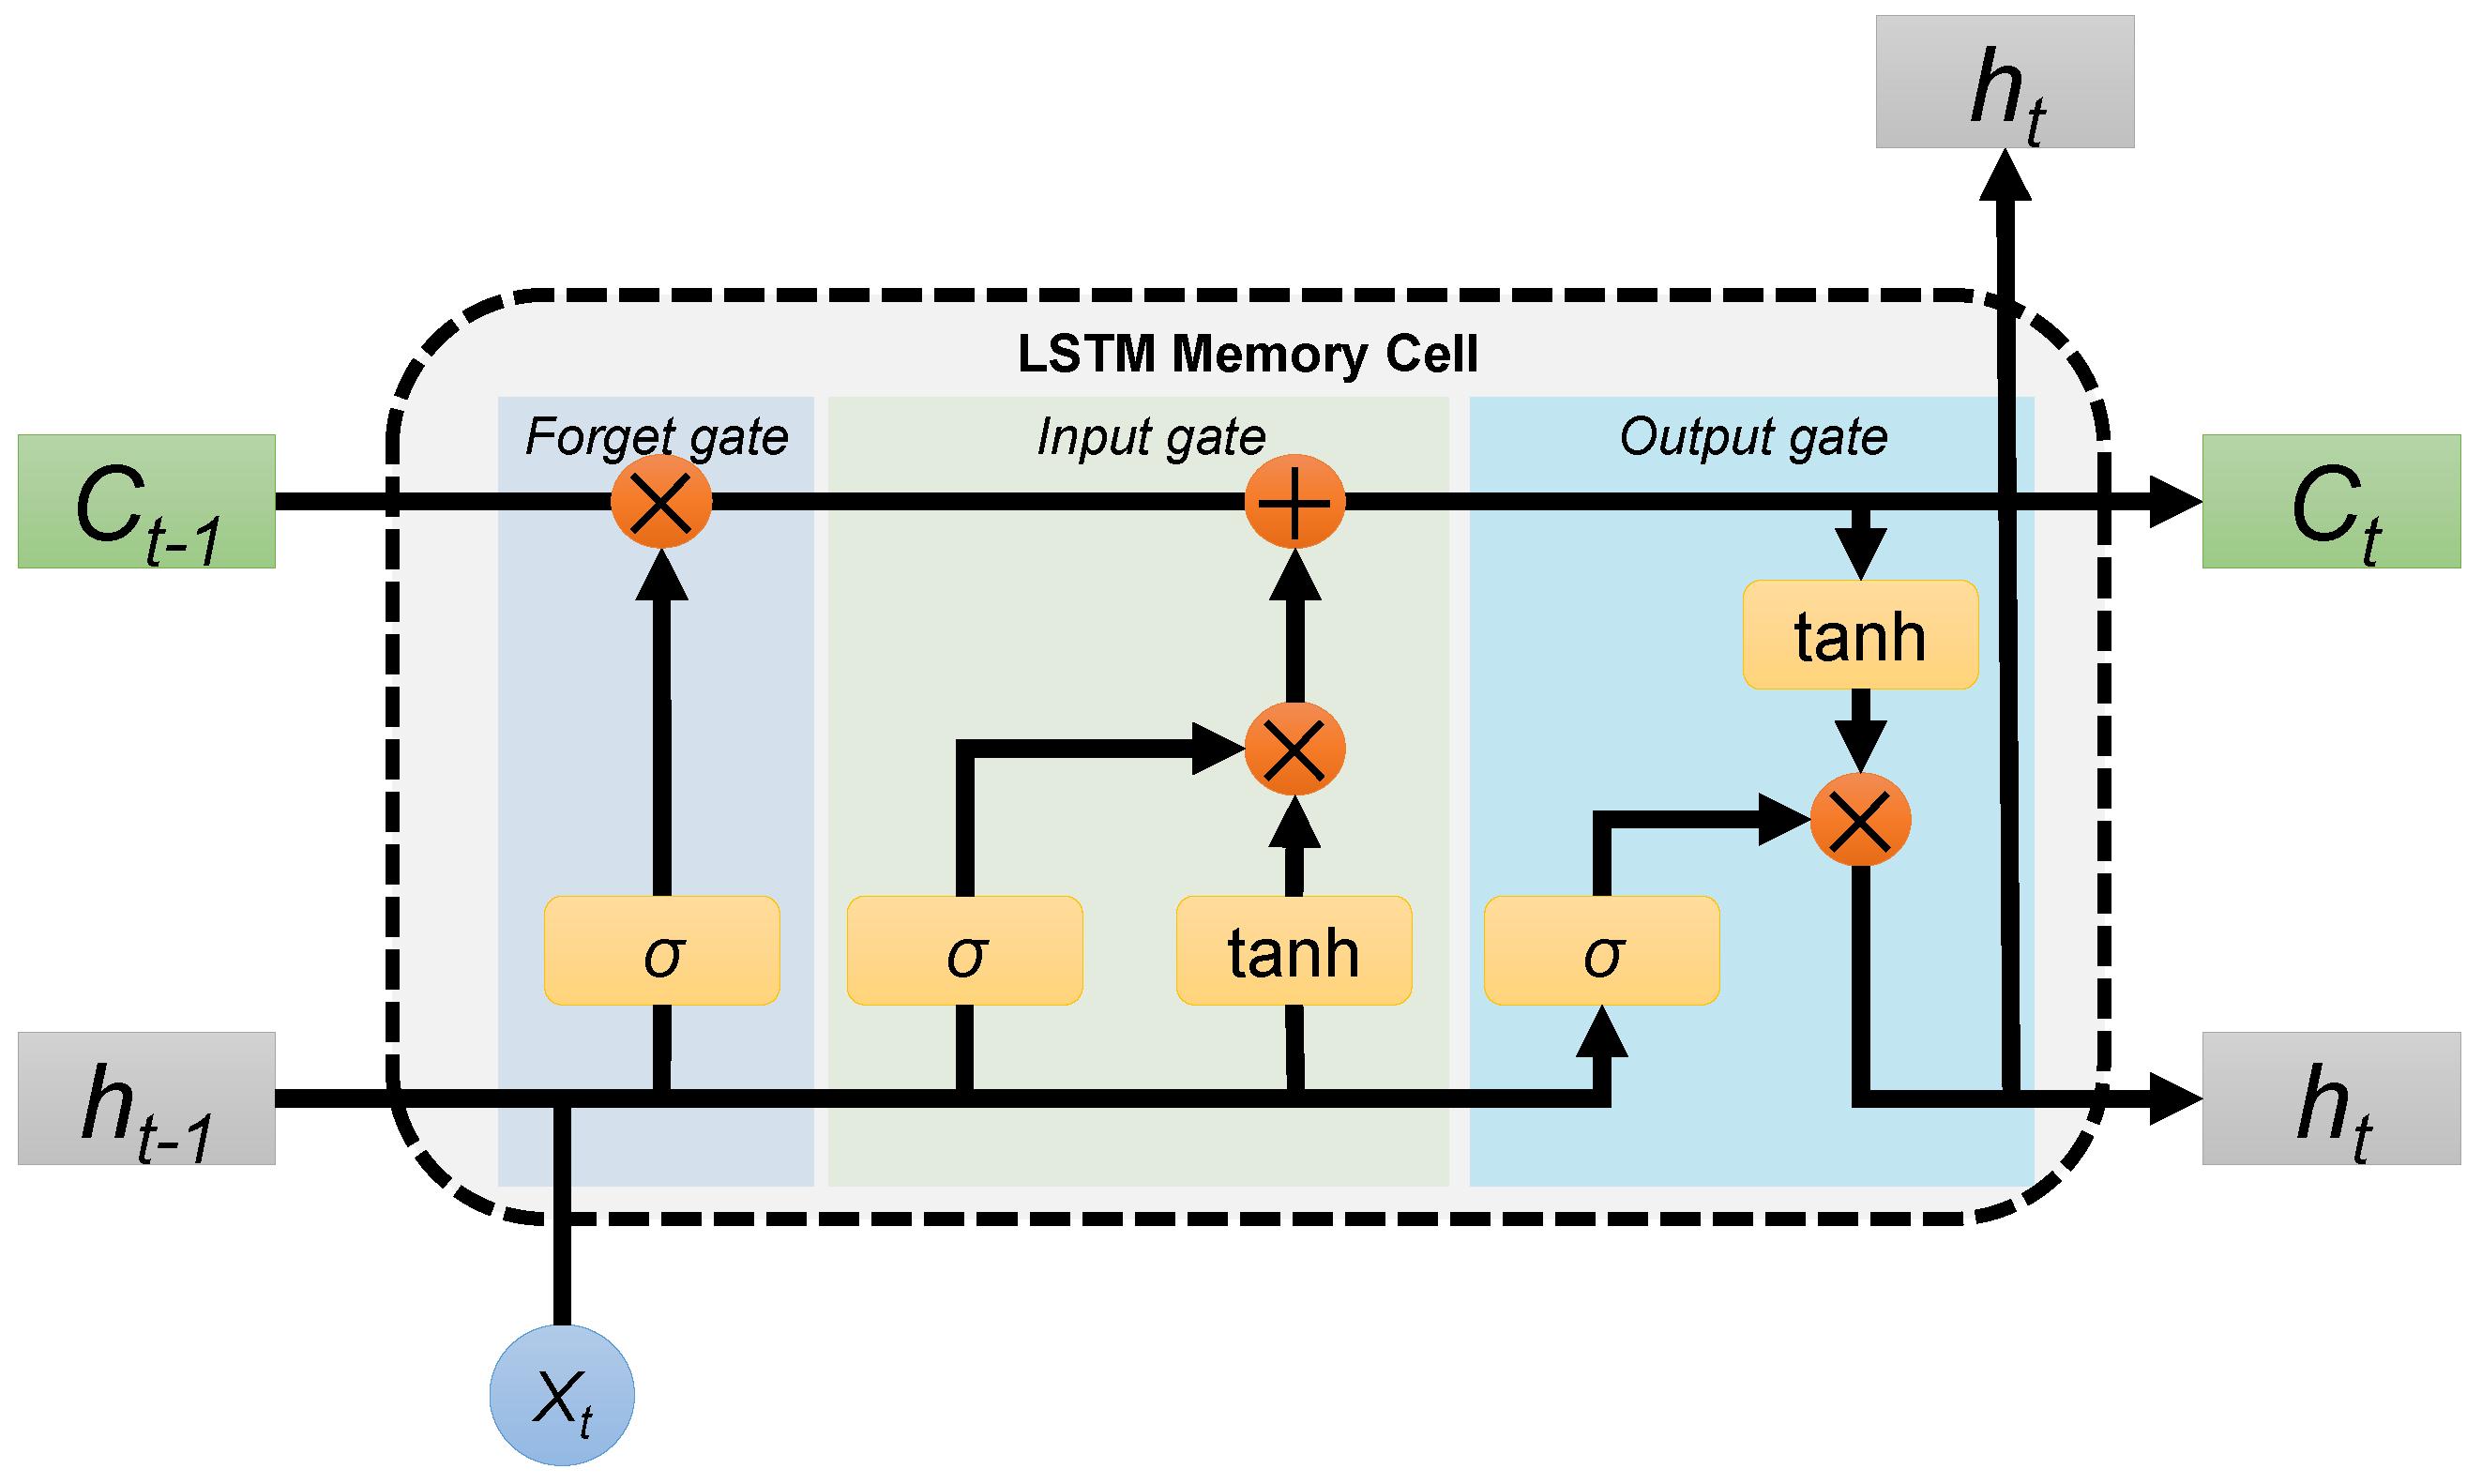
\includegraphics[width=0.70\linewidth]{LSTM.png}
  \caption{Схема работы LSTM-ячейки.}
\end{figure}

\subsubsection*{Основные элементы}
На каждом временном шаге \(t\):
\begin{itemize}
  \item \(x_t\) - входной вектор (например, значение временного ряда в момент \(t\));
  \item \(h_{t-1}\) - предыдущее скрытое состояние (краткосрочная память);
  \item \(C_{t-1}\) - предыдущее состояние ячейки (долгосрочная память);
  \item \(h_t\) - новое скрытое состояние;
  \item \(C_t\) - обновлённое состояние ячейки.
\end{itemize}

Каждый вентиль управляет потоком данных через сигмоидную функцию \(\sigma(x)=1/(1+e^{-x})\), возвращающую значения от 0 до 1, где 0 - «закрыт» (ничего не пропускать), а 1 - «открыт» (пропускать всё).
Для нелинейного преобразования информации используется \(\tanh(x)\), сжимающий значения в диапазон \((-1, 1)\).


\subsubsection*{Формулы LSTM}

\textbf{1. Вентиль забывания (Forget gate):}
\[
f_t = \sigma(W_f x_t + U_f h_{t-1} + b_f)
\]
Этот вентиль контролирует, какая часть предыдущей памяти \(C_{t-1}\) сохраняется.
Если компонент \(f_t^i \approx 1\), $i$-я ячейка памяти остаётся почти неизменной; если \(f_t^i \approx 0\), её содержимое забывается.

\textbf{2. Вентиль входа (Input gate):}
\[
i_t = \sigma(W_i x_t + U_i h_{t-1} + b_i)
\]
Определяет, сколько новой информации попадёт в память.

\textbf{3. Кандидат на обновление памяти (Candidate cell):}
\[
\tilde{C}_t = \tanh(W_C x_t + U_C h_{t-1} + b_C)
\]
Этот вектор содержит «новое содержание» памяти - то, что сеть *предлагает* записать, если входной вентиль разрешит.

\textbf{4. Обновление состояния памяти (Cell state update):}
\[
C_t = f_t \odot C_{t-1} + i_t \odot \tilde{C}_t
\]
Это ключевое уравнение LSTM: старое состояние \(C_{t-1}\) частично сохраняется, частично обновляется новой информацией.
Благодаря этому прямому пути (почти линейному) градиент может свободно течь назад во времени, не затухая.

\textbf{5. Вентиль выхода (Output gate):}
\[
o_t = \sigma(W_o x_t + U_o h_{t-1} + b_o)
\]
Решает, какая часть обновлённого состояния \(C_t\) будет передана наружу в скрытое состояние \(h_t\).

\textbf{6. Вычисление нового скрытого состояния:}
\[
h_t = o_t \odot \tanh(C_t)
\]
Это "наблюдаемое" состояние, участвующее в генерации прогноза.

\subsubsection*{Пошаговый процесс вычислений (пример на временном ряде)}

Рассмотрим временной ряд \( \{y_1, y_2, \ldots, y_T\} \), и пусть задача - на каждом шаге предсказать следующее значение \( \hat{y}_{t+1} \).

\begin{enumerate}
  \item \textbf{Инициализация:}
  Задаём $h_0 = 0$ и $C_0 = 0$.
  Модель пока ничего не «помнит» - память пуста.

  \item \textbf{Первый шаг ($t=1$): вход $x_1=y_1$.}
  \begin{align*}
  f_1 &= \sigma(W_f x_1 + U_f h_0 + b_f),\\
  i_1 &= \sigma(W_i x_1 + U_i h_0 + b_i),\\
  \tilde{C}_1 &= \tanh(W_C x_1 + U_C h_0 + b_C),\\
  C_1 &= f_1 \odot C_0 + i_1 \odot \tilde{C}_1,\\
  o_1 &= \sigma(W_o x_1 + U_o h_0 + b_o),\\
  h_1 &= o_1 \odot \tanh(C_1).
  \end{align*}
  Теперь память \(C_1\) содержит информацию о первом наблюдении, а $h_1$ можно использовать для прогноза $\hat{y}_2 = W_y h_1 + b_y$.

  \item \textbf{Второй шаг ($t=2$): вход $x_2=y_2$.}
  Текущее состояние зависит от предыдущего:
  \begin{align*}
  f_2 &= \sigma(W_f x_2 + U_f h_1 + b_f),\\
  i_2 &= \sigma(W_i x_2 + U_i h_1 + b_i),\\
  \tilde{C}_2 &= \tanh(W_C x_2 + U_C h_1 + b_C),\\
  C_2 &= f_2 \odot C_1 + i_2 \odot \tilde{C}_2,\\
  o_2 &= \sigma(W_o x_2 + U_o h_1 + b_o),\\
  h_2 &= o_2 \odot \tanh(C_2).
  \end{align*}
  Таким образом, новое состояние \(C_2\) - это комбинация памяти о первом и втором наблюдениях, с учётом того, что могло быть частично забыто через \(f_2\).

  \item \textbf{Дальнейшие шаги.}
  Для $t=3,\dots,T$ повторяются те же операции.
  Модель адаптивно решает, какие части истории важны. Например:
  \begin{itemize}
    \item если ряд стабилен, $f_t \approx 1$ - память сохраняется;
    \item при смене режима $f_t$ падает, а $i_t$ растёт - старая информация стирается, новая записывается;
    \item $o_t$ регулирует силу отклика на выходе - в моменты «шума» он может частично блокировать передачу состояния.
  \end{itemize}
\end{enumerate}


\subsubsection*{Итоговая логика работы}
В каждый момент времени LSTM делает три вещи:
\begin{enumerate}
  \item \textbf{Сохраняет} полезную информацию в памяти (\(f_t\));
  \item \textbf{Обновляет} память новыми сведениями (\(i_t, \tilde{C}_t\));
  \item \textbf{Формирует} выход, основанный на текущем контексте (\(o_t\)).
\end{enumerate}

Такой механизм обеспечивает контролируемый баланс между «долгой» и «краткой» памятью.
Благодаря этому LSTM умеет учитывать зависимости на десятки и даже сотни шагов, что делает её одной из базовых архитектур для прогнозирования временных рядов, обработки текста и анализа сигналов.






\subsection{Упрощённые рекуррентные блоки GRU}

Архитектура \textbf{GRU (Gated Recurrent Unit)} была предложена как более компактная альтернатива LSTM.
Она сохраняет ключевую идею — контролировать поток информации через вентили, — но делает это с меньшим числом параметров и без отдельного состояния памяти \( C_t \).
GRU объединяет долгосрочную и краткосрочную память в одно скрытое состояние \( h_t \), что упрощает вычисления и ускоряет обучение, при этом практически не уступая LSTM по качеству.

\begin{figure}[h]
  \centering
  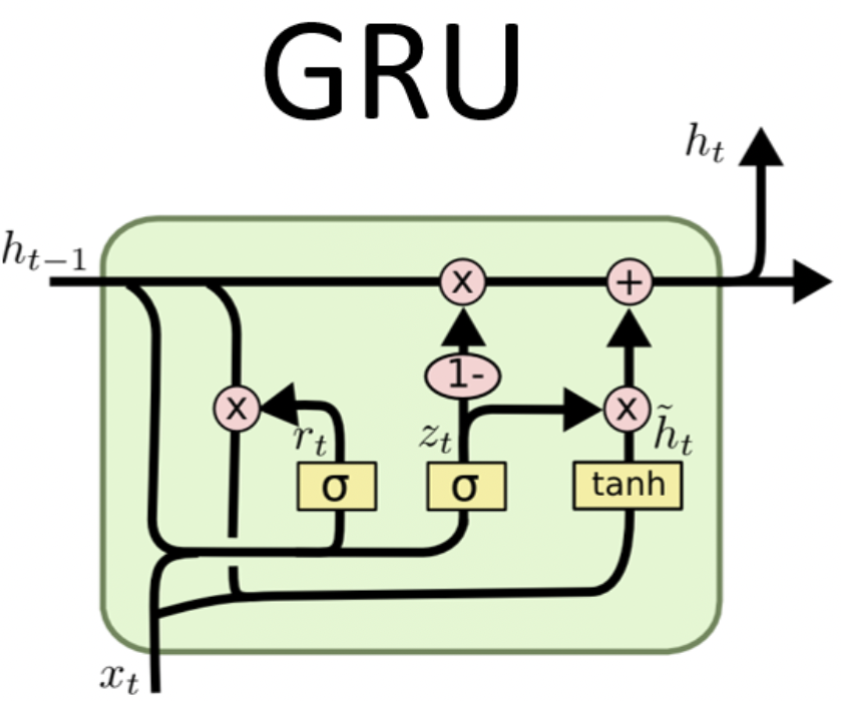
\includegraphics[width=0.5\linewidth]{GRU.png}
  \caption{Схема блока GRU: вентиль обновления $z_t$, вентиль сброса $r_t$, кандидаты нового состояния $\tilde{h}_t$ и итоговое скрытое состояние $h_t$.}
\end{figure}

\subsubsection*{Основная идея}
GRU использует два вентиля:
\begin{itemize}
  \item \textbf{Вентиль обновления} \( z_t \) — решает, сколько старой информации сохранить в новом состоянии;
  \item \textbf{Вентиль сброса} \( r_t \) — управляет тем, насколько учитывать предыдущее состояние при формировании нового кандидата.
\end{itemize}


\subsubsection*{Формулы GRU}

\textbf{1. Вентиль обновления (Update gate):}
\[
z_t = \sigma(W_z x_t + U_z h_{t-1} + b_z)
\]
Если \( z_t \) близок к 1 — модель сохраняет большую часть старого состояния; если близок к 0 — состояние полностью обновляется.

\textbf{2. Вентиль сброса (Reset gate):}
\[
r_t = \sigma(W_r x_t + U_r h_{t-1} + b_r)
\]
Определяет, какую долю предыдущей информации нужно «сбросить» при вычислении нового кандидата.

\textbf{3. Кандидат нового состояния:}
\[
\tilde{h}_t = \tanh\!\bigl(W_h x_t + U_h (r_t \odot h_{t-1}) + b_h\bigr)
\]
Если \(r_t \approx 0\), прошлое состояние почти не влияет на \(\tilde{h}_t\), то есть модель полностью «забывает» старую информацию и создаёт новое представление из текущего входа.

\textbf{4. Итоговое скрытое состояние (обновление памяти):}
\[
h_t = (1 - z_t) \odot h_{t-1} + z_t \odot \tilde{h}_t
\]
Это взвешенная комбинация старого состояния \(h_{t-1}\) и нового кандидата \(\tilde{h}_t\).
Если \(z_t\) велико, сеть обновляется сильно; если мало — «помнит» старое состояние.


\subsubsection*{Интуитивное объяснение}
GRU можно рассматривать как динамический фильтр:
\begin{itemize}
  \item \(r_t\) решает, сколько прошлого контекста учитывать при обновлении;
  \item \(z_t\) решает, насколько вообще менять текущее состояние;
  \item \(\tilde{h}_t\) создаёт новую информацию, а итоговое \(h_t\) аккуратно «смешивает» старое и новое знание.
\end{itemize}
Таким образом, GRU самостоятельно регулирует глубину своей памяти без необходимости хранить отдельный вектор \( C_t \), как в LSTM.

\subsubsection*{Пошаговый процесс вычислений (пример на временном ряде)}

Пусть дан временной ряд \( \{y_1, y_2, \ldots, y_T\} \).
На каждом шаге \(t\) сеть получает вход \(x_t = y_t\) и предыдущее состояние \(h_{t-1}\).

\begin{enumerate}
  \item \textbf{Инициализация:} \(h_0 = 0.\)
  \item \textbf{Шаг $t=1$: вход $x_1$.}
  \begin{align*}
    z_1 &= \sigma(W_z x_1 + U_z h_0 + b_z),\\
    r_1 &= \sigma(W_r x_1 + U_r h_0 + b_r),\\
    \tilde{h}_1 &= \tanh(W_h x_1 + U_h (r_1 \odot h_0) + b_h),\\
    h_1 &= (1 - z_1) \odot h_0 + z_1 \odot \tilde{h}_1.
  \end{align*}
  Теперь $h_1$ — это «память» сети о первом наблюдении, адаптивно отфильтрованная вентилями.

  \item \textbf{Шаг $t=2$: вход $x_2$.}
  \begin{align*}
    z_2 &= \sigma(W_z x_2 + U_z h_1 + b_z),\\
    r_2 &= \sigma(W_r x_2 + U_r h_1 + b_r),\\
    \tilde{h}_2 &= \tanh(W_h x_2 + U_h (r_2 \odot h_1) + b_h),\\
    h_2 &= (1 - z_2) \odot h_1 + z_2 \odot \tilde{h}_2.
  \end{align*}
  Таким образом, сеть адаптирует память: если $z_2$ мало, она «помнит» прошлое; если велико — обновляется новыми сведениями.

  \item \textbf{Дальнейшие шаги ($t=3,\ldots,T$):} процесс повторяется.
  GRU динамически управляет тем, насколько сильно прошлое влияет на текущее предсказание.
\end{enumerate}


\subsubsection*{Сравнение с LSTM}

\begin{itemize}
  \item GRU имеет только два вентиля против трёх у LSTM и не использует отдельное состояние ячейки \(C_t\); память и выход объединены в \(h_t\).
  \item За счёт меньшего числа параметров GRU обучается быстрее и требует меньше данных.
  \item На длинных последовательностях LSTM может обеспечивать чуть более стабильное запоминание, однако в большинстве практических задач GRU демонстрирует сопоставимую точность.
\end{itemize}

Таким образом, GRU — это более простая, но эффективная альтернатива LSTM, сохраняющая ключевую способность моделировать долгосрочные зависимости во временных рядах.



\section{Encoder-Decoder, attention}

\subsection{Seq2Seq как ступень к вниманию}

\paragraph{От анализа последовательностей к их генерации}
Рекуррентные нейронные сети доказали эффективность в задачах анализа последовательностей, однако такие постановки предполагают фиксированную структуру выхода. Во многих же практических задачах требуется сформировать последовательность заранее неизвестной длины. Машинный перевод — наиболее яркий пример: длина перевода может отличаться от длины исходной фразы, а соответствие между словами двух языков редко бывает прямым и однозначным. Это естественно приводит к идее архитектуры, которая не только обрабатывает последовательность, но и генерирует новую.

\paragraph{Архитектура encoder--decoder}
Подход sequence-to-sequence основан на паре взаимодополняющих модулей: \textit{энкодера}, который преобразует входную последовательность в компактное скрытое представление, и \textit{декодера}, который по этому представлению порождает выходную последовательность:
\[
x=(x_1,\dots,x_T) \quad\longrightarrow\quad c \quad\longrightarrow\quad y=(y_1,\dots,y_N).
\]
В качестве основного строительного блока в классическом варианте используются рекуррентные сети: LSTM или GRU.

\paragraph{Работа энкодера и декодера}
Энкодер считывает токены по одному, обновляя скрытое состояние
\[
h_t = f_{\mathrm{enc}}(x_t, h_{t-1}),\quad t=1,\dots,T,
\]
после чего финальное состояние $h_T$ принимается в роли контекстного вектора $c$. На практике возможны более развитые варианты агрегации, включая двунаправленные слои.
Декодер инициализируется функцией от $c$:
\[
s_0 = g(c),
\]
и далее генерирует выход авто-регрессионно:
\[
s_n = f_{\mathrm{dec}}(y_{n-1}, s_{n-1}, c), \qquad
p(y_n \mid x, y_{<n}) = \mathrm{Softmax}(W_o s_n + b_o).
\]
Генерация начинается со специального токена начала последовательности $\langle \mathrm{bos} \rangle$ и продолжается до появления токена окончания $\langle \mathrm{eos} \rangle$ либо достижения допустимой длины.

\paragraph{Ограничение контекстного представления}
Такое устройство накладывает фундаментальное ограничение: вся информация о входе концентрируется в одном фиксированного размера векторе $c$. При работе с длинными или содержательно насыщенными последовательностями это приводило к утрате важных деталей, особенно тех, что оказываются востребованными на поздних шагах генерации. Отсюда и снижение качества на длинных предложениях и зависимость результата от длины и структуры входа.

\paragraph{Тонкости применения}
На каждом шаге предсказывается распределение $p(y_n \mid x, y_{<n})$ по словарю. Простая стратегия выбора наиболее вероятного токена работает не всегда оптимально, так как локальный максимум может вести к глобально нежелательной последовательности. В практических системах для улучшения качества вывода используют beam search, поддерживая несколько наиболее вероятных кандидатов и сравнивая их по
\[
\max_{y_{1:n}} \prod_{t=1}^{n} p(y_t \mid x, y_{<t}).
\]

\begin{figure}[h]
  \centering
  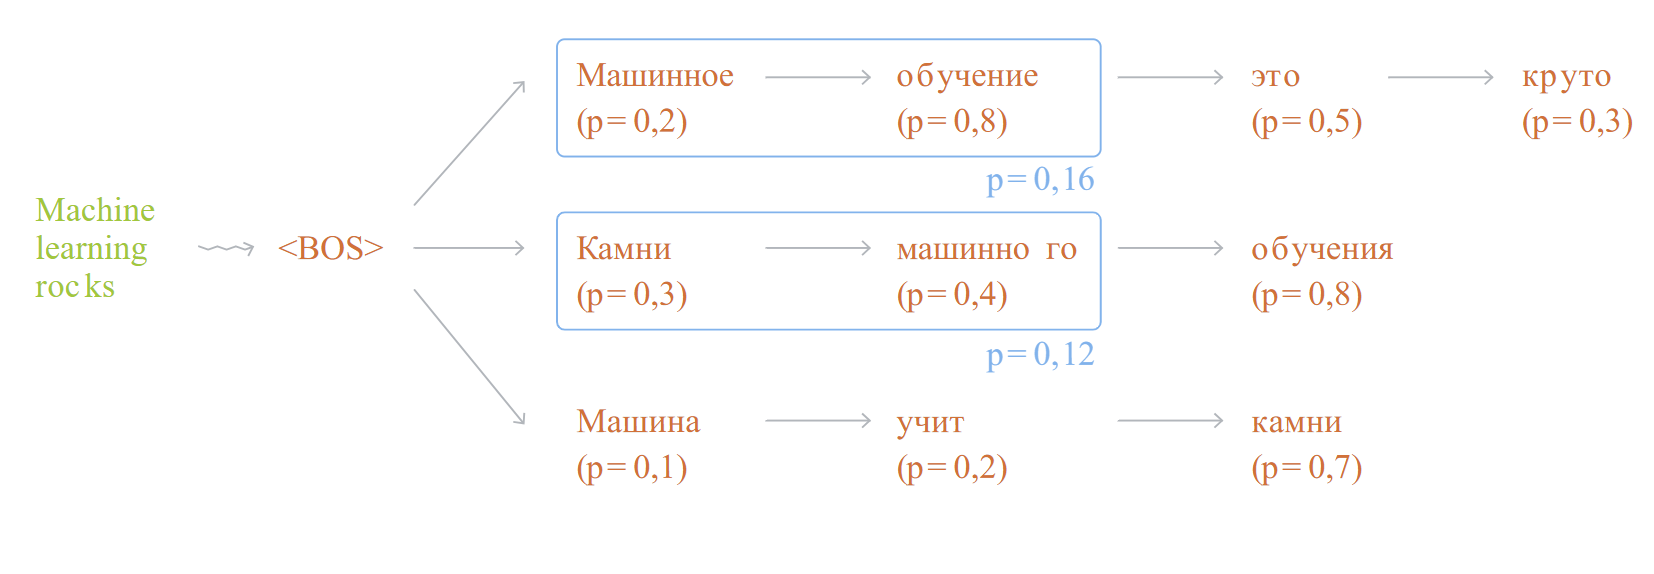
\includegraphics[width=0.70\linewidth]{Seq2Seq.png}
  \caption{Тонкости применения seq2seq, машинный перевод}
\end{figure}

\paragraph{Тонкости обучения и teacher forcing}
Последовательность оптимизируется по суммарной кросс-энтропии
\[
\mathcal{L} = -\sum_{n=1}^{N} \log p\bigl(y^{\ast}_n \mid x, y^{\ast}_{<n}\bigr),
\]
где $y^{\ast}$ — истинная разметка.
Одна из сложностей такого обучения состоит в том, что, единожды ошибившись и предсказав неправильный
$\hat{y}^{(n)}$
вместо истинного
$y^{(n)}$,
модель, скорее всего, и следующие токены предскажет неверно. Это сделает всё дальнейшее обучение малополезным: ведь мы будем учить декодер предсказывать правильное продолжение неправильного начала.

Одним из способов борьбы с этим является \textit{teacher forcing}. Суть его в том, что на этапе обучения мы подаём на вход декодера не предсказанный им на предыдущем этапе токен, а истинный.


\paragraph{One-to-many постановки}
Архитектура encoder--decoder естественна для задач вида one-to-many, где входовое представление сводится к одному контексту, а на выходе требуется сформировать целую последовательность. Помимо машинного перевода, примером служит генерация подписей к изображениям: вектор признаков, извлечённый свёрточной сетью, можно использовать как контекст для декодера, обучая всю систему end-to-end.


\subsection{Механизм внимания (attention)}

Классическая архитектура encoder--decoder концентрирует всю информацию о входе в одном контекстном векторе. На практике это затрудняет генерацию длинных и структурно сложных последовательностей: разные части входа имеют разную значимость, и при генерации разных фрагментов выхода модель должна учитывать разные фрагменты исходной последовательности.

Механизм внимания реализует естественную для человека стратегию: на каждом шаге декодирования модель «смотрит» на те элементы входа, которые важны именно для текущего предсказания. Рассмотрим классическую формулировку внимания по Bahdanau et al. (2014).

\paragraph{Обозначения}
Пусть энкодер сформировал набор скрытых представлений
\[
H = (h_1,\dots,h_T), \qquad h_j \in \mathbb{R}^{d_h},
\]
а декодер генерирует выход по шагам
\[
s_i \in \mathbb{R}^{d_s}, \qquad i = 1,\dots,N.
\]
Инициализация состояния декодера обычно проводится через контекстный вектор, например $s_0 = h_T$.

\paragraph{Веса внимания и динамический контекст}
На шаге $i$ декодер сравнивает своё текущее состояние $s_i$ с каждым $h_j$, вычисляя \emph{оценки внимания}:
\[
e_{i,j} = \mathrm{score}(s_i, h_j).
\]
Пусть $e_i = (e_{i,1},\dots,e_{i,T})$ — вектор этих оценок. Нормируем его с помощью softmax:
\[
\alpha_i = \mathrm{softmax}(e_i),
\]
где $\alpha_{i,j}$ показывает, насколько важна позиция $j$ входа при порождении токена $y_i$.

Затем строим \emph{контекстный вектор} для шага $i$:
\[
a_i = \sum_{j=1}^{T} \alpha_{i,j}\, h_j.
\]
Этот вектор аккумулирует релевантную информацию о входе для текущего шага декодера. Для получения выходного представления используют конкатенацию или аффинное преобразование:
\[
\tilde{s}_i = \tanh\!\bigl(W_c [s_i; a_i] + b_c\bigr), \qquad
p(y_i \mid x,y_{<i}) = \mathrm{Softmax}(W_o \tilde{s}_i + b_o).
\]

\paragraph{Варианты score-функций}
Используются несколько стандартных форм:
\[
\text{(аддитивное, Bahdanau)}\quad
e_{i,j}=v^\top \tanh(W_s s_i + W_h h_j + b),
\]
\[
\text{(мультипликативное, Luong)}\quad
e_{i,j}= s_i^\top W h_j,
\qquad
\text{(скалярное произведение)}\quad
e_{i,j}= s_i^\top h_j.
\]
Все варианты совместимы с общей схемой, различаясь гибкостью и вычислительной эффективностью.

\paragraph{Интерпретация}
Вектор $\alpha_i$ является распределением внимания по токенам входа: большие веса указывают на те элементы последовательности, которые оказываются контекстно значимыми для предсказания текущего выхода $y_i$.

Благодаря пересчёту $a_i$ на каждом шаге, декодер получает содержательный доступ ко всему следу энкодера и может фокусироваться на разных частях входа в зависимости от текущего шага генерации. Такой механизм устраняет необходимость в единственном фиксированном контексте и значительно улучшает качество seq2seq-моделей.




\subsection{Self-attention (внутреннее внимание)}

Механизм внимания оказался полезен не только в декодере, но и на стороне энкодера.
Self-attention позволяет каждому токену, формируя своё представление, учитывать остальные токены входной последовательности, мгновенно находя между ними смысловые связи.
Такой подход был предложен в архитектуре Transformer (Vaswani et al., 2017) и стал ключевым шагом к моделям, эффективно работающим с длинными зависимостями.

\paragraph{Query, Key и Value}
Пусть входная последовательность преобразована в матрицу эмбеддингов
\[
X =
\begin{bmatrix}
x_1^\top \\
\vdots \\
x_T^\top
\end{bmatrix}
\in \mathbb{R}^{T \times d_{\text{model}}}.
\]
Для каждого токена строятся три проекции:
\[
Q = X W^Q,\qquad
K = X W^K,\qquad
V = X W^V,
\]
где $W^Q,W^K,W^V$ — обучаемые матрицы.
Интуитивно:
\begin{itemize}
\item $Q$: «куда направлено внимание» (запрос),
\item $K$: «кто привлекает внимание» (ключ),
\item $V$: «что передаётся» (значение).
\end{itemize}

\paragraph{Вычисление внимания}
Для каждого токена $i$ сравниваем его запрос $q_i$ со всеми ключами:
\[
\text{score}_{ij} = \frac{q_i k_j^\top}{\sqrt{d_k}}.
\]
Преобразуем оценки в веса внимания:
\[
\alpha_{ij} = \mathrm{softmax}(\text{score}_{ij}),
\]
затем вычисляем новое представление токена $i$:
\[
\text{output}_i = \sum_{j=1}^{T} \alpha_{ij} v_j.
\]

В матричной форме всё внимание вычисляется сразу:
\[
\mathrm{SelfAttn}(Q, K, V)
=
\mathrm{softmax}
\left(
\frac{QK^\top}{\sqrt{d_k}}
\right)V.
\]

\paragraph{Multi-head self-attention}
Разные типы зависимостей удобно выделять раздельно.
Поэтому внимание считают параллельно в $H$ головах:
\[
\mathrm{head}_h =
\mathrm{softmax}
\left(
\frac{Q_h K_h^\top}{\sqrt{d_k}}
\right)
V_h,
\quad h=1,\dots,H,
\]
где проекции выполняются отдельными матрицами $W_h^Q, W_h^K, W_h^V$.
После вычислений головы конкатенируются:
\[
\mathrm{MHA}(X) =
\mathrm{Concat}(\mathrm{head}_1,\dots,\mathrm{head}_H)\,W^O.
\]

\begin{figure}[h]
  \centering
  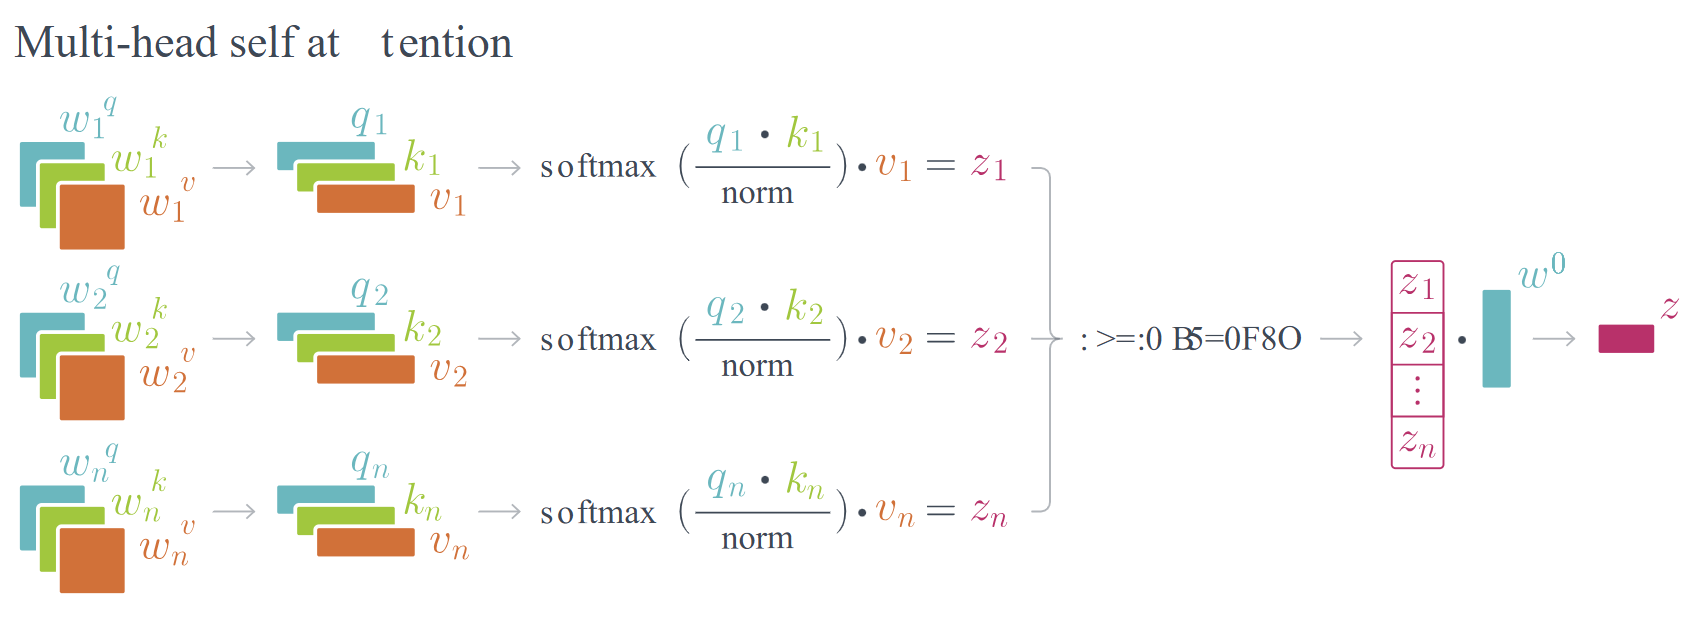
\includegraphics[width=0.70\linewidth]{MHA.png}
  \caption{Схема вычисления multi-head self-attention}
\end{figure}

Так модель учится выделять разные зависимости: синтаксис, семантику,
отношения объект–действие, дальние ссылки и многое другое.

\paragraph{Маскирование}
В задачах авторегрессии (например, языковое моделирование, прогнозирование временных рядов) модель не должна использовать будущие токены.
Поэтому перед softmax вводят \textit{причинную маску} $M$:
\[
M_{ij} =
\begin{cases}
0, & j \le i, \\
-\infty, & j > i,
\end{cases}
\]
и вычисление внимания принимает вид:
\[
A =
\mathrm{softmax}
\left(
\frac{QK^\top}{\sqrt{d_k}} + M
\right).
\]
Значения $-\infty$ обнуляются после softmax, запрещая связь с будущими позициями.

Маскирование применяется \emph{до} объединения голов, обеспечивая корректное поведение каждой self-attention головы в авторегрессионном режиме.

\paragraph{Итог}
Self-attention позволяет токенам напрямую взаимодействовать друг с другом, формируя контекстуализованные представления без длинных путей передачи информации, свойственных RNN.
Благодаря чисто матричной природе вычислений слой эффективно параллелится и стал фундаментом современных трансформеров.



\subsection{Трансформеры}

Трансформер объединяет уже знакомые нам механизмы \textit{self-attention}, \textit{multi-head attention} и причинное маскирование в единый вычислительный блок, который легко масштабируется и хорошо параллелится. Ключевая идея — отказаться от последовательного «переноса» информации через скрытое состояние (как в RNN) и дать каждой позиции прямой доступ ко всему контексту за один слой, а затем локально преобразовать полученное представление.

\begin{figure}[h]
  \centering
  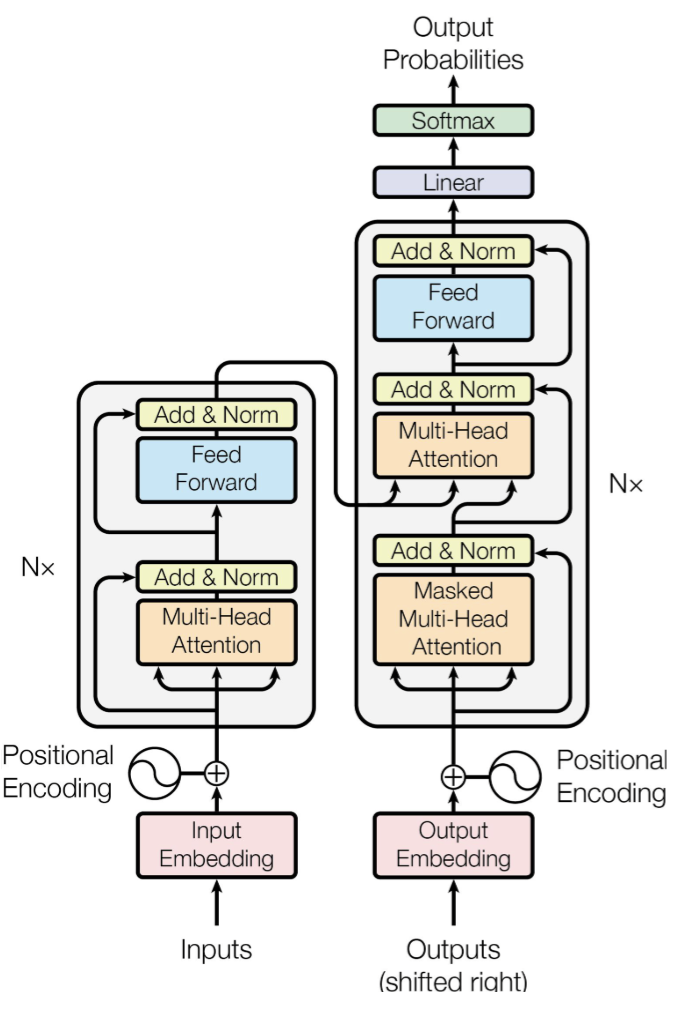
\includegraphics[width=0.60\linewidth]{transformer.png}
  \caption{Архитектура Transformer: стек энкодер-блоков и стек декодер-блоков}
\end{figure}

\paragraph{Поток данных от входа к выходу}
\begin{enumerate}\itemsep0.2em
  \item \textbf{Входные эмбеддинги и позиции} \quad
  Токены преобразуются в эмбеддинги $E$ и складываются с позиционными представлениями $P$, чтобы модель различала порядок:
  \[
  X_0 = \mathrm{Embed}(\text{токены}) + P.
  \]
  Позиции кодируют либо фиксированными синусоидами
  \[
  \mathrm{PE}(\text{pos},2i)=\sin\!\Bigl(\frac{\text{pos}}{10000^{2i/d}}\Bigr),\quad
  \mathrm{PE}(\text{pos},2i{+}1)=\cos\!\Bigl(\frac{\text{pos}}{10000^{2i/d}}\Bigr),
  \]
  либо обучаемыми абсолютными/относительными эмбеддингами.
  \item \textbf{Стек энкодер-блоков} \quad
  Каждый блок получает $X$ и возвращает тензор той же длины:
  \[
  X \xrightarrow{\;\mathrm{MHA}\;} \tilde X \xrightarrow{\;\mathrm{Add\ \&\ LayerNorm}\;} X' \xrightarrow{\;\mathrm{FFN}\;} \tilde Z \xrightarrow{\;\mathrm{Add\ \&\ LayerNorm}\;} Z.
  \]
  \item \textbf{Стек декодер-блоков (для генерации)} \quad
  Последовательность шагов в одном блоке:
  \[
  Y \xrightarrow{\;\mathrm{Masked\ MHA}\;} \tilde Y \xrightarrow{\;\mathrm{Add\ \&\ LN}\;} Y'
  \xrightarrow{\;\mathrm{Cross\text{-}Attn}(Q{=}Y',\,K{=}Z_{\text{enc}},\,V{=}Z_{\text{enc}})\;}
  \tilde U \xrightarrow{\;\mathrm{Add\ \&\ LN}\;} U
  \xrightarrow{\;\mathrm{FFN}\;} \tilde V \xrightarrow{\;\mathrm{Add\ \&\ LN}\;} V.
  \]
  Здесь $Z_{\text{enc}}$ — выход энкодера, а masked MHA использует причинную маску, запрещающую доступ к будущим позициям.
\end{enumerate}

\paragraph{Multi-Head Self-Attention в блоке}
Мы уже вывели формулу внимания:
\[
\mathrm{SelfAttn}(Q,K,V)=\mathrm{softmax}\!\left(\frac{QK^\top}{\sqrt{d_k}}\right)V.
\]
В блоке применяется параллельно $H$ голов; результаты конкатенируются и проецируются обратно:
\[
\mathrm{head}_h=
\mathrm{softmax}\!\left(\frac{Q_hK_h^\top}{\sqrt{d_k}}\right)V_h,
\qquad
\mathrm{MHA}(X)=\mathrm{Concat}(\mathrm{head}_1,\ldots,\mathrm{head}_H)W^O.
\]
MHA даёт гибкость: разные головы подхватывают локальные, дальние, синтаксические и семантические зависимости.

\paragraph{Position-wise Feed-Forward}
После сбора контекста внимание передаёт по позициям «обогащённые» векторы, но взаимодействие между признаками внутри одного токена по-прежнему линейно. За нелинейные преобразования отвечают одинаковые для всех позиций полносвязные слои:
\[
\mathrm{FFN}(x)=\phi(xW_1+b_1)\,W_2+b_2.
\]
Где:
\begin{itemize}
  \item \textit{позиционность}: FFN действует независимо для каждой позиции, без смешивания токенов, поэтому отвечает не за «сбор контекста», а за «перемешивание признаков» внутри токена;
  \item \textit{размерности}: промежуточное пространство обычно в $3$–$4$ раза шире $d_{\text{model}}$ (часто обозначают $d_{\text{ff}}$);
  \item \textit{нелинейность}: исторически использовали ReLU, сегодня чаще \textit{GELU} с формой $\phi(x)\approx x\,\Phi(x)$, что даёт более гладкую сходимость;
  \item \textit{стоимость}: при коротких последовательностях именно FFN может доминировать по FLOPs и памяти, несмотря на квадратичность внимания.
\end{itemize}
Интуитивно блок работает как «сначала собрать нужный контекст по всей последовательности» (MHA), затем «сильно переработать представление внутри токена» (FFN).

\paragraph{Нормализация и остаточные связи}
Каждый подблок обёрнут в схему \textit{Add \& LayerNorm}, что стабилизирует тренинг и обеспечивает прохождение градиента через глубину. Нормализуется \emph{каждый токен отдельно по его признакам} (feature dimension), а не по батчу и не по времени. Это важно:
\begin{itemize}
  \item разные длины последовательностей и паддинги нарушают статистики по времени/батчу;
  \item токены семантически неоднородны, их нельзя «усреднять» друг с другом;
  \item при авторегрессивном инференсе (GPT-подобные модели) LayerNorm не зависит от будущих токенов и работает одинаково при $batch{=}1$;
  \item BatchNorm требует стабильной батч-статистики, чего в NLP обычно нет.
\end{itemize}
Существуют две расстановки нормализации:
\begin{itemize}
  \item \textbf{Post-LN}: $\mathrm{LayerNorm}(x+\mathrm{SubLayer}(x))$ — историческая версия оригинальной статьи;
  \item \textbf{Pre-LN}: $x+\mathrm{SubLayer}(\mathrm{LayerNorm}(x))$ — как правило, устойчивее при увеличении числа слоёв благодаря лучшему градиентному потоку.
\end{itemize}

\paragraph{Энкодер, декодер и кросс-внимание}
Энкодер обрабатывает вход двунаправленно: self-attention не ограничен маской и может использовать всю последовательность. Декодер работает авторегрессионно: masked self-attention запрещает «видеть будущее», а слой cross-attention сопоставляет текущий контекст декодера с представлениями энкодера, извлекая релевантные фрагменты источника при генерации.

\paragraph{Шаблоны использования и предобученные семейства}
\textbf{Encoder-only} (\textit{BERT}-подобные) модели используют двунаправленный self-attention и решают задачи понимания: классификация, извлечение сущностей, поиск, re-ranking. Предобучение обычно включает:
\begin{enumerate}\itemsep0pt
  \item \textit{Masked Language Modeling (MLM)} — случайные токены заменяются на [MASK], модель восстанавливает их по контексту;
  \item \textit{Next Sentence Prediction (NSP)} — по паре фрагментов нужно определить, следует ли второй за первым.
\end{enumerate}
\textbf{Decoder-only} (\textit{GPT}-подобные) модели — это стек декодеров с причинной маской; обучаются как языковые модели по задаче «следующий токен». Такой формат естественно поддерживает генерацию и все задачи, редуцируемые к ней (суммаризация, диалог, код, пошаговое предсказание).

\paragraph{Сложность и длинные последовательности}
Self-attention оценивает все пары позиций, что даёт $O(T^2)$ по времени и памяти. Это цена за прямой доступ ко всему контексту и полную параллелизацию. Для очень длинных входов применяют локальные/разреженные схемы внимания, иерархические уровни, а также техники сжатия или «patchification», которые снижают затраты при сопоставимом качестве.

\paragraph{Итог}
Трансформерный блок — это последовательность операций, где \textit{MHA} собирает контекст по всей последовательности, \textit{FFN} нелинейно перерабатывает признаки внутри токена, а \textit{Add \& LayerNorm} обеспечивает стабильность и глубину. В связке энкодер–декодер архитектура естественно решает seq2seq-задачи; в encoder-only и decoder-only вариантах — масштабируется под понимание и генерацию соответственно

\section{Метрики оценки качества}

При прогнозировании временных рядов и при порождении текстовых последовательностей используются разные группы метрик, поскольку отличаются типы выходных данных модели. В этом разделе рассмотрим наиболее употребимые оценки.

\subsection{Метрики для регрессионного прогноза временных рядов}

Пусть $y_t$ — истинное значение временного ряда на шаге $t$, $\hat y_t$ — предсказание модели, $T$ — число оцениваемых точек. Наиболее распространённые ошибки:

\paragraph{MAE (Mean Absolute Error)}
\[
\mathrm{MAE} =
\frac{1}{T}\sum_{t=1}^{T} |y_t - \hat y_t|.
\]
Интерпретируется в тех же единицах, что и сам ряд. Устойчивее к выбросам, чем MSE.

\paragraph{MSE и RMSE (Mean Squared Error / Root MSE)}
\[
\mathrm{MSE} = \frac{1}{T}\sum_{t=1}^{T} (y_t - \hat y_t)^2,
\qquad
\mathrm{RMSE} = \sqrt{\mathrm{MSE}}.
\]
Сильнее штрафуют крупные ошибки; удобны для оптимизации (квадратичный лосс).

\paragraph{MAPE (Mean Absolute Percentage Error)}
\[
\mathrm{MAPE} = \frac{100\%}{T}\sum_{t=1}^{T}
\left|\frac{y_t - \hat y_t}{y_t}\right|.
\]
Показывает относительную ошибку в процентах. Плохо работает при $y_t\approx0$.

\paragraph{SMAPE (Symmetric MAPE)}
\[
\mathrm{SMAPE} = \frac{100\%}{T}
\sum_{t=1}^{T}
\frac{|y_t - \hat y_t|}{(|y_t| + |\hat y_t|)/2}.
\]
Снижает влияние малых $y_t$ по сравнению с MAPE.

\paragraph{WAPE (Weighted Absolute Percentage Error)}
\[
\mathrm{WAPE} =
\frac{\sum_{t=1}^{T} |y_t - \hat y_t|}
{\sum_{t=1}^{T} |y_t|}.
\]
Полезен при больших различиях в масштабе данных; часто используется в ритейле.

\subsection{Метрики вероятностного прогноза}

Для моделей, предсказывающих распределения или интервалы неопределённости:

\paragraph{Quantile (Pinball) Loss}
Для квантиля $\tau \in (0,1)$:
\[
L_\tau (y_t, \hat y_t) =
\max\bigl(\tau (y_t - \hat y_t),(\tau-1)(y_t - \hat y_t)\bigr).
\]
Применяется в multi-horizon прогнозировании для построения предиктивных интервалов.

\paragraph{CRPS (Continuous Ranked Probability Score)}
\[
\mathrm{CRPS}(F, y) =
\int_{-\infty}^{+\infty}
\bigl(F(z) - \mathbf{1}\{z \ge y\}\bigr)^2 dz,
\]
где $F$ — предсказанное распределение. Оценивает качество вероятностного прогноза целиком.

\subsection{Метрики для оценки качества текста (NLP)}

При генерации последовательностей чаще оценивают не числовую ошибку, а точность воспроизведения содержания и структуры текста. Пусть $G$ — гипотеза (сгенерированный текст), $R$ — эталон.

\paragraph{BLEU (Bilingual Evaluation Understudy)}
Оценка n-граммного совпадения при машинном переводе:
\[
\mathrm{BLEU} =
\mathrm{BP}
\cdot
\exp\!\left(\sum_{n=1}^{N} w_n \log p_n\right),
\]
где $p_n$ — точность по $n$-граммам, $\mathrm{BP}$ — brevity penalty (штраф за слишком короткий перевод).

\paragraph{ROUGE (Recall-Oriented Understudy for Gisting Evaluation)}
Чаще применяется в суммаризации. Например,
\[
\mathrm{ROUGE\text{-}L} =
\frac{(1+\beta^2)\cdot \mathrm{R}\cdot \mathrm{P}}
{\mathrm{R} + \beta^2 \mathrm{P}},
\]
где $\mathrm{R}$ и $\mathrm{P}$ — полнота и точность по LCS (длина наибольшей общей подпоследовательности).

\paragraph{METEOR}
Вычисляется по словам с учётом лемматизации и синонимов:
\[
\mathrm{METEOR} =
(1 - \mathrm{penalty}) \cdot F_{\mathrm{mean}},
\]
что делает её чувствительнее к перефразировкам, чем BLEU.

\paragraph{Perplexity (PP)}
\[
\mathrm{PP} =
\exp\left(
-\frac{1}{T}\sum_{t=1}^{T}
\log p(y_t \mid y_{<t})
\right).
\]
Характеризует способность языковой модели предсказывать следующий токен. Чем меньше, тем лучше.

\paragraph{Accuracy (для классификации токенов)}
\[
\mathrm{Acc} =
\frac{1}{T}
\sum_{t=1}^{T}
\mathbf{1}\{\hat y_t = y_t\}.
\]
Используется, например, при задаче Masked Language Modeling в BERT.

\medskip
Подбор метрик зависит от типа задачи: регрессионный прогноз временных рядов требует числовых ошибок (MAE, MAPE), генерация текста — содержательных оценок (BLEU, ROUGE), а вероятностный прогноз — оценок распределений (Pinball, CRPS).


\section{Актуальные наборы данных}

Ниже собраны популярные наборы данных для прогнозирования временных рядов и для оценки seq2seq-моделей в NLP. Для каждого указаны краткое описание, формат, типичная постановка задачи и ссылка.

\paragraph{M4 Competition Dataset}
\begin{itemize}
  \item \textbf{Описание.} 100{,}000+ временных рядов различных частот (год, квартал, месяц, неделя, день, час) из экономики, демографии, финансов и др.
  \item \textbf{Формат.} Исторические траектории с фиксированным горизонтом прогноза (6--18 шагов в зависимости от частоты).
  \item \textbf{Задача.} Многогоризонтное прогнозирование $y_{T+1:T+H}$ по истории $y_{1:T}$; сравнение статистических и DL-подходов.
  \item \textbf{Ссылка.} \href{https://www.kaggle.com/datasets/yogesh94/m4-forecasting-competition-dataset}{https://www.kaggle.com/datasets/yogesh94/m4-forecasting-competition-dataset}
\end{itemize}

\paragraph{Electricity Load Diagrams}
\begin{itemize}
  \item \textbf{Описание.} Почасовое электропотребление множества абонентов; классический панельный временной ряд.
  \item \textbf{Формат.} Сотни серий с одинаковой частотой; возможны календарные признаки.
  \item \textbf{Задача.} Прогноз нагрузки по объектам (multi-series), в т. ч. с общими параметрами модели.
  \item \textbf{Ссылка.} \href{https://www.kaggle.com/datasets/uciml/electric-power-consumption-data-set}{https://www.kaggle.com/datasets/uciml/electric-power-consumption-data-set}
\end{itemize}

\paragraph{Traffic (дорожный трафик)}
\begin{itemize}
  \item \textbf{Описание.} Измерения трафика/потока автомобилей по сенсорам; используется для краткосрочного прогноза.
  \item \textbf{Формат.} Многомерные ряды (сенсоры) с равномерной частотой (минуты/часы), календарные признаки.
  \item \textbf{Задача.} Прогноз трафика на горизонте $H$ для каждого сенсора; часто multi-horizon и multi-series.
  \item \textbf{Ссылка.} \href{https://www.kaggle.com/datasets/pooriamst/metro-interstate-traffic-volume}{https://www.kaggle.com/datasets/pooriamst/metro-interstate-traffic-volume}
\end{itemize}

\paragraph{Weather / Climate (погодные измерения)}
\begin{itemize}
  \item \textbf{Описание.} Метеопараметры (температура, давление, влажность, ветер) во времени; используются для кратко/среднесрочного прогноза.
  \item \textbf{Формат.} Один или несколько каналов с часовыми/минутными метками, возможны пропуски.
  \item \textbf{Задача.} Прогноз погодных величин (например, температуры) на горизонте $H$; оценка вероятностных интервалов.
  \item \textbf{Ссылка.} \href{https://www.kaggle.com/datasets/mnassrib/jena-climate}{https://www.kaggle.com/datasets/mnassrib/jena-climate}
\end{itemize}

\paragraph{WMT14 En--De (машинный перевод)}
\begin{itemize}
  \item \textbf{Описание.} Классический корпус для обучения и оценки систем перевода «английский↔немецкий».
  \item \textbf{Формат.} Параллельные предложения (source--target), стандартные разбиения train/valid/test.
  \item \textbf{Задача.} Seq2seq-перевод; оценка BLEU/TER/ROUGE для сравнения энкодер--декодер/Transformer-моделей.
  \item \textbf{Ссылка.} \href{http://www.statmt.org/wmt14/translation-task.html}{http://www.statmt.org/wmt14/translation-task.html}
\end{itemize}

\paragraph{CNN/DailyMail (суммаризация)}
\begin{itemize}
  \item \textbf{Описание.} Новости и рефераты к ним; стандарт для абстрактной и экстрактивной суммаризации.
  \item \textbf{Формат.} Пары (статья, реферат), десятки тысяч примеров.
  \item \textbf{Задача.} Seq2seq-суммаризация; оценка ROUGE-1/2/L, METEOR, иногда BERTScore.
  \item \textbf{Ссылка.} \href{https://www.kaggle.com/datasets/sunnysai12345/news-summary}{https://www.kaggle.com/datasets/sunnysai12345/news-summary}
\end{itemize}


\section{Обзор литературы}

Развитие методов прогнозирования последовательностей прослеживается через ряд фундаментальных исследований, каждое из которых вносило ключевой вклад в улучшение качества обработки данных со сложными временными и структурными зависимостями.

\subsection{Классические статистические методы}
\begin{itemize}
  \item \textbf{Hyndman, Athanasopoulos (2018). Forecasting: Principles and Practice.}
  \href{https://otexts.com/fpp3/}{Ссылка}
  Систематический фундамент по прогнозированию временных рядов. Обсуждаются методы экспоненциального сглаживания, ARIMA и их сезонные расширения, модели с экзогенными переменными.
  Представлены практические эксперименты на экономических и демографических данных: демонстрация того, что корректный выбор сезонности и стационаризации критически влияет на точность прогноза.
\end{itemize}

\subsection{Рекуррентные нейронные сети}
\begin{itemize}
  \item \textbf{Rumelhart et al. (1986). Learning Representations by Back-Propagating Errors.}
  \href{https://www.nature.com/articles/323533a0}{Ссылка}
  Первые эксперименты с RNN показывают способность модели запоминать краткосрочные зависимости, но выявляют серьёзную проблему исчезающих и взрывающихся градиентов при длинных последовательностях.

  \item \textbf{Hochreiter, Schmidhuber (1997). Long Short-Term Memory.}
  \href{https://www.bioinf.jku.at/publications/older/2604.pdf}{Ссылка}
  Предлагается архитектура LSTM с механизмом «вентилей памяти». В экспериментах демонстрируется успешное извлечение дальних зависимостей на синтетических задачах (например, «долгая память») и значительное превосходство над классическими RNN в задачах речи.

  \item \textbf{Cho et al. (2014). Learning Phrase Representations Using RNN Encoder–Decoder for SMT.}
  \href{https://arxiv.org/abs/1406.1078}{Ссылка}
  Вводит GRU и схему encoder–decoder для машинного перевода. В экспериментах модель улучшает качество перевода по сравнению со статистическими SMT-системами, особенно на предложениях переменной длины.
\end{itemize}

\subsection{Attention,seq2seq и Трансформеры}
\begin{itemize}
  \item \textbf{Bahdanau, Cho, Bengio (2014). Neural Machine Translation by Jointly Learning to Align and Translate.}
  \href{https://arxiv.org/abs/1409.0473}{Ссылка}
  Предлагается механизм внимания: декодер динамически определяет важные части входного предложения на каждом шаге.
  Эксперименты: повышение BLEU для длинных предложений, интерпретируемость через матрицы «выравнивания» (attention maps).
  \item \textbf{Vaswani et al. (2017). Attention Is All You Need.}
  \href{https://arxiv.org/abs/1706.03762}{Ссылка}
  Полный переход к self-attention, отказ от рекуррентности.
  Эксперименты: на задаче WMT14 English–German Transformer превосходит тогдашние SOTA модели по BLEU при значительно **быстрейшем обучении**, особенно на больших данных.

  \item \textbf{Devlin et al. (2018). BERT: Pre-training of Deep Bidirectional Transformers.}
  \href{https://arxiv.org/abs/1810.04805}{Ссылка}
  Показано, что двунаправленное внимание улучшает понимание языка.
  Эксперименты: значительный скачок качества на GLUE и SQuAD; MLM и NSP позволяют эффективно использовать неразмеченные тексты.

  \item \textbf{Radford et al. (2018–2020). GPT Series: Generative Pretrained Transformers.}
  \href{https://cdn.openai.com/research-covers/language-unsupervised/language_understanding_paper.pdf}{Ссылка на GPT-1}
  Стек декодеров для генерации текста.
  Эксперименты: улучшение perplexity на языковом моделировании, появление zero-shot возможностей в GPT-2/3 на широком спектре задач.
\end{itemize}

\subsection{Практические источники}
\begin{itemize}
  \item \textbf{Хендбук Яндекса по машинному обучению}
  \href{https://education.yandex.ru/handbook/ml}{Ссылка}
  Практическое изложение моделей seq2seq, внимания и трансформеров с примерами. Использовался как опорный материал при подготовке данного доклада.
\end{itemize}

В совокупности эти исследования демонстрируют последовательный прогресс: от анализа временных рядов простыми статистическими методами до глубоких моделей с вниманием и масштабируемыми трансформерными архитектурами, которые доминируют в современных задачах прогнозирования и генерации последовательностей.


\end{document}
